\chapter{Introduction}
The following document is a dissertation for my final year project in which I hope to achieve a B.Sc. (Hons.) in Software Development. This project was undertaken by just myself and all work shown is my own.

From the beginning of the year I knew I wanted to make a practical web application, a website that could actually be useful to people and would also provide me with a suitable challenge and rewarding, worthwhile learning outcomes. Much research went into what kind of project I would do and what technologies I would use to do it which will be discussed further on in the document.

The finished project however is a job site for software developers. I opted to use mainly React, a Javascript library for the front-end along with some accompanying frameworks and used Spring Boot for the back-end as well as MongoDB for the database.

\section{Early Research}
Initially the project was going to take a much different shape in my mind. I had planned on it being more of a general purpose 'odd-job' type app where users could post or accept listings advertising a certain amount of pay for menial jobs such as mowing a lawn or cleaning up around a house etc.

As the idea grew in my head I realised I would prefer it to be specific to my field of study. I decided my project would be a job site specifically for software developers. This way I could incorporate OAuthentification into the website with developers logging in via their LinkedIn or even Github accounts. This would tie in nicely to the general theme and purpose of the website. OAuth doesn't share password data but instead uses authorization tokens to prove an identity between consumers and service providers. OAuth is an authentication protocol that allows you to approve one application interacting with another on your behalf without giving away your password \cite{OAuth}.

\subsection{MEAN Stack}
I had initially planned on developing the project using the MEAN stack. The MEAN stack (MongoDB, Express.js, AngularJS and Node.js) is a free and open-source JavaScript software stack for building dynamic web sites and web applications \cite{mean}. Because all components of the MEAN stack support programs that are written in JavaScript, MEAN applications can be written in one language for both server-side and client-side execution environments. However, after discussing it with my supervisor, I learned that this might not have appeared challenging enough to some as it had already been covered in the previous year. A big part of the applied project is to showcase self learning and the ability to understand foreign concepts that haven't been explicitly taught in class. Although I joined this year after 2 years out of college I agreed it would be better if I tried to show technologies not already covered on the curriculum and weren't seen before among this group of students.

\subsection{MERN Stack}
After deciding against the MEAN stack, I looked into the MERN stack (MongoDB, Express, React, and Node. js), again however, there wasn't really enough variation in language and I would have been making a glorified JavaScript application.

\subsection{Dropwizard \& Spring Boot}
I decided I was trying too hard to conform to a predefined 'stack' and realised I didn't have to choose a set of technologies that work well together just because they form a nice acronym. I wanted to have a back-end built in a language other than JavaScript and for developing RESTful web services you don't need to look much farther than DropWizard or Spring Boot.

\subsubsection{Dropwizard}
Dropwizard is a Java framework for developing web services in Java. Dropwizard makes use of multiple different packages such as \textbf{Jetty, Jersey and Jackson} that let you deploy a micro-service with relative ease\cite{dropwizard}. On top of that, we were actually using Dropwizard in our first semester for the module 'Distributed Systems' so I would have had the added help of knowledge gained from these assignments.

\subsubsection{Spring Boot}
The other technology I looked into was Spring Boot. Like Dropwizard, Boot makes it all too easy to get a Java web application up and running in mere minutes. Spring Boot is a Spring framework module which provides Rapid Application Development (RAD) feature to the Spring framework. It is highly dependent on the starter templates feature which is very powerful and works flawlessly \cite{boot:howto}.

I did a lot of research into these two technologies and found that I was only one of a great many developers unsure about which one to go for. There are countless articles and websites online going into great details comparing the two frameworks and I found it quite easy to get bogged down by an overload of information on the two (Figure ~\ref{drop_label}). In the end I opted for Spring Boot, I found examples of how well it interacts with MongoDB and decided that would be very useful in my application. I don't think development of the API would have suffered at all had I gone for Dropwizard, they're both clearly two very popular technologies for Java web development.

\begin{figure}[h]
    \centering
    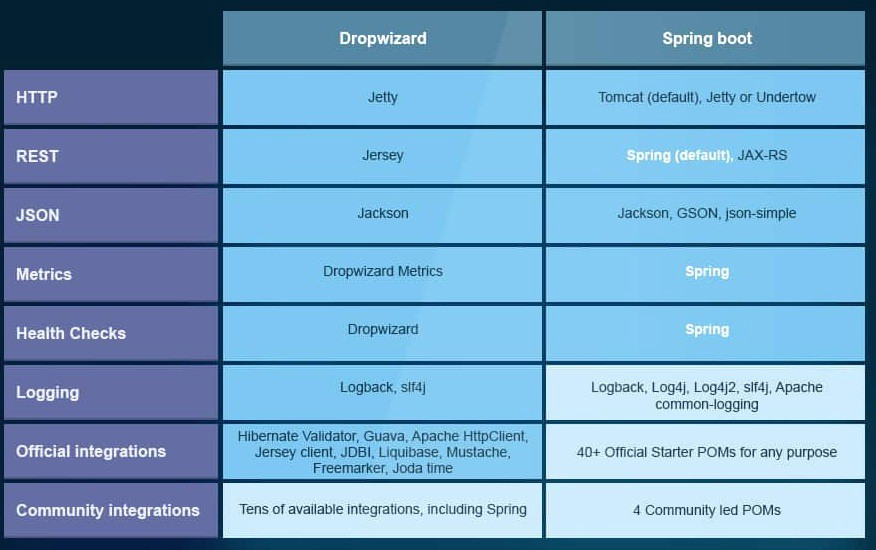
\includegraphics[scale=0.3]{Images/dropwizard.jpeg} 
    \label{drop_label}
    \caption{Comparison of 3rd party libraries}
\end{figure}

\section{What the Project Brings}
The premise of the project as touched on above, was to bring a small number of technologies together, and have them working efficiently and effectively with a clear reason for their use. As it was just myself in the group, I was generally happy for the scope to be a bit smaller as long as the project itself was an effective program functioning well across different levels in the stack.

The 3 main technologies effectively offer everything a web application would need to be deployed and used by an actual user.

\section{Scope}
As mentioned earlier, I developed the project by myself. Taking this into consideration I felt that a full stack application, hosted online was suitably challenging. The project's architecture consists of three unique tiers all communicating in a stack to form the web application. The three parts are as follows: 

\subsection{Database/Back-End Tier}
I used MongoDB for my database technology. MongoDB is a NoSQL database, it is document oriented and it stores data in collections instead of tables \cite{parker2013comparing}. The main use of the database is to store my job objects. The users of my application can perform basic CRUD functionality on the jobs stored in the database. My MongoDB database is hosted on a cloud service called MongoDB Atlas. This is done so that when they application is deployed online via Heroku, the data is available at all times.

\subsection{Server Side/Middle Tier}
For my 'middle' tier I used Spring Boot. Spring Boot is a fantastic variation of Spring that allows for quick painless development of a web application with almost no configuration. The RESTful API is contained in my Spring server and connects the React application to the Mongo database containing the job objects to be manipulated. The REST API is hosted as its own application on Heroku and communicates with the React application to perform requests.

A deciding factor in choosing Spring boot as my server side technology was it's very powerful MongoDB connector. All you need to do is simply extend the 'MongoRepository' class from a repository interface which contains plenty of generic methods already. Impressively, you do not need to manually implement these queries yourself, instead you can use Spring Boot's repository naming conventions, and the 'MongoRepository' will intelligently construct the queries at run-time \cite{marchioni2015mongodb}.

\subsection{Front-End Tier}
For the front end of my web application I decided to use React. React is a Javascript library for building UI's. However, as it is only concerned with rendering data to the DOM. React requires  additional libraries for state management, sending HTTP requests and routing such as React Router and Axios \cite{wiki:xxx}. I use multiple Javascript libraries in my application to compliment React such and will examine them later in the document.

I performed testing on the front-end application using two testing frameworks, 'Jest' and 'React-Testing-Library'.

\section{Objectives}
Like the vast majority of students in my year, my primary objective in developing this application was to learn a new set of skills and to become familiar with a new set of technologies. It was also a great opportunity to develop and improve my project management skills as it demands attention over an extended period of time. I believe by choosing technologies I have had no substantial previous experience with I definitely accomplished this objective. I set the following goals for my project from the very beginning of the year:

\begin{itemize}
    \item I wanted my application to have a number of moving parts and to be a real 'Full Stack Application'. I felt a 3 tier system would go a long way towards showing me how a production ready application might actually look in the working world. When developing across different levels you learn a lot about how each level of the stack works, how they communicate with each other, what works well together and what doesn't.
    \item As I have a big interest in web development in particular, I specifically wanted to become very familiar with React. According to Stack Overflow's 2019 survey, more developers say they use React.js than Angular, a switch from last year \cite{Stack}. It ranked second overall behind JQuery.
    \item Adding to what I said earlier about getting a taste for what a real world application might look, I felt it was very important to have genuine authentication. I initially wanted OAuthentication but opted instead for JSON Web Tokens or failing that, basic authentication.
    \item I wanted users to be able to perform the basic CRUD functionalities with jobs.
    \item I wanted the application to be deployed on Heroku.

\end{itemize}

\section{Documentation}
This document will give a detailed description of my research, planning, reasoning and thought process throughout the development of my application. It is split up into six chapters. Each detailing a different aspect of the work put into the application itself. They are: 

    \subsubsection{Introduction}
    The current chapter, the introduction, has covered what my aims for the project were early on. What research I did before choosing to develop using the technologies I did and also my objectives for the project before beginning development.
    
    \subsubsection{Methodology}
    This chapter will go over how I went about the development of my project at a more detailed level. It will cover how often I met with my supervisor and how often I dedicated each week to the project. It will essentially cover how I went about developing and planning the entire project, which project methodology was used and if I felt it was at the right level. 
    
    \subsubsection{Technology Review}
    This chapter will documents the outcome of my research into the technologies I used and how I used them to achieve my objectives. Every technology used in the development of the application will be described here, covering what they do in general and what they offer to my application specifically.
    
    \subsubsection{System Design}
    This section will describe the architecture of the application. It will cover how each tier of the application communicate together to form the complete project. It will contain diagrams and screenshots to help visualise the structure and architecture of the application.
    
    \subsubsection{System Evaluation}
    In this chapter I will do a full evaluation of the application as a whole. I will compare the final outcome of the application with the objectives I initially outlined in the Introduction chapter. I will also outline any limitations or difficulties I found in the project be it through technologies used or through my own decisions and mistakes. I will also suggest improvements I believe could be made on the application.
    
    \subsubsection{Conclusion}
    The conclusion will be a summary of the entire finished project. It will discuss my initial goals for the project and how well I managed to achieve them. I will cover what I feel I learned throughout the development of the project and the writing of the dissertation. It will also outline any regrets I have with the project be they from using the wrong technologies or other matters. Overall I hope it will provide a final piece of insight on my experience with the project and hopefully wrap up the documentation.